\chapter{Introduction}

This introductory chapter aims to present the general context which wraps this project, going in some depth inside \textit{deep learning and robotics}. We will also amble along some of the latest advances and most useful current applications of the junction between these two fields. Lastly, we will situate this project on the previously described context. After this chapter, each key aspect of the work flow will be further explained.\\

\section{Robots}

Robotics applications can be really useful at daily tasks. These tasks are of greater interest when the behavioral of a robot tends to emulate the human one\footnote{\href{https://www.engadget.com/2018/01/08/new-sony-aibo-first-impressions/}{Some efforts are taken even into adopting the performance of human's best friend}}, with the advantage of no human people exposed to a significant risk, or, in a less gloomy scenario, without human body physical limitations. This requires a polished (and somehow complex) behavioral, which is triggered by a certain input. At this point, we can find two main branches into robots, depending on the input source:
\begin{itemize}
	\item \textbf{Teleoperated robots:} this kind of robots are capable of perform certain actions, which are \textit{remotely controlled by a human operator}. This application is the one with most weight on the hazardousness (\autoref{fig:1_pioneer}) \cite{chernobyl-robot} or precision \cite{teleop-surgery} factor. Thus, some advances are made nowadays improving the teleoperation function, implementing \emph{feedbacks} from the robot, such as haptic feedback \cite{teleop-haptic}, or VR (\emph{Virtual Reality}) sensation, to allow that person to sense the environment as if it was in front of it.	
	
	\item \textbf{Autonomous robots:} these robots are much more complex machines, as they are distinguished for implementing a response by itself, independently of any kind of remote operator. This is seeked on certain scenarios, where there are some factors (as the time elapsed performing an action, or the cost of a control link with the robot) with a considerable weight in the design \cite{ai-space}. This is the kind of robots that concern us on this work: the state-of-the-art techniques try to emulate \emph{human behavioral}(\autoref{fig:1_pepper}), so some actions can begin to be performed with a certain intelligence, as we will describe below.
\end{itemize}


	\begin{figure}[h]
		\centering
		\begin{subfigure}[b]{0.4\textwidth}
			\centering
			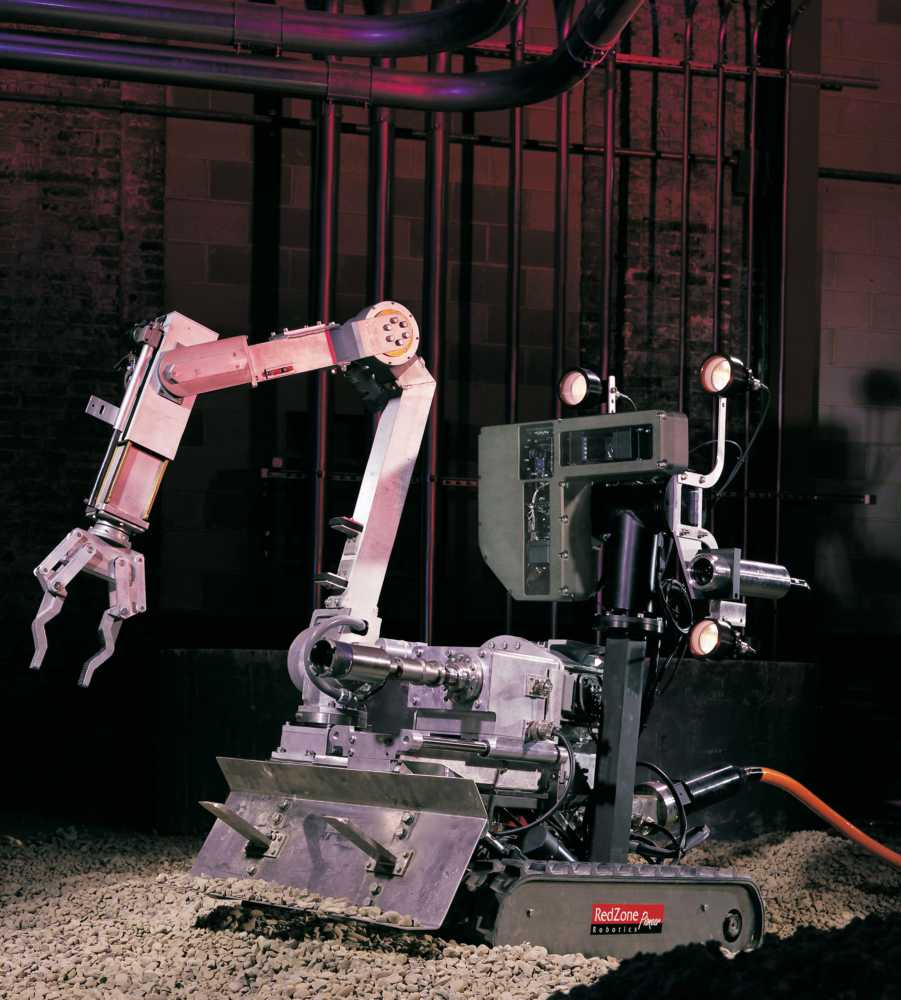
\includegraphics[width=0.8\linewidth]{images/pioneer_chernobyl}
			\caption{Pioneer robot, designed to perform hazardous teleoperated explorations in a deadly radioactive environment.}
			\label{fig:1_pioneer}
		\end{subfigure}
		\hfill
		\begin{subfigure}[b]{0.4\textwidth}
			\centering
			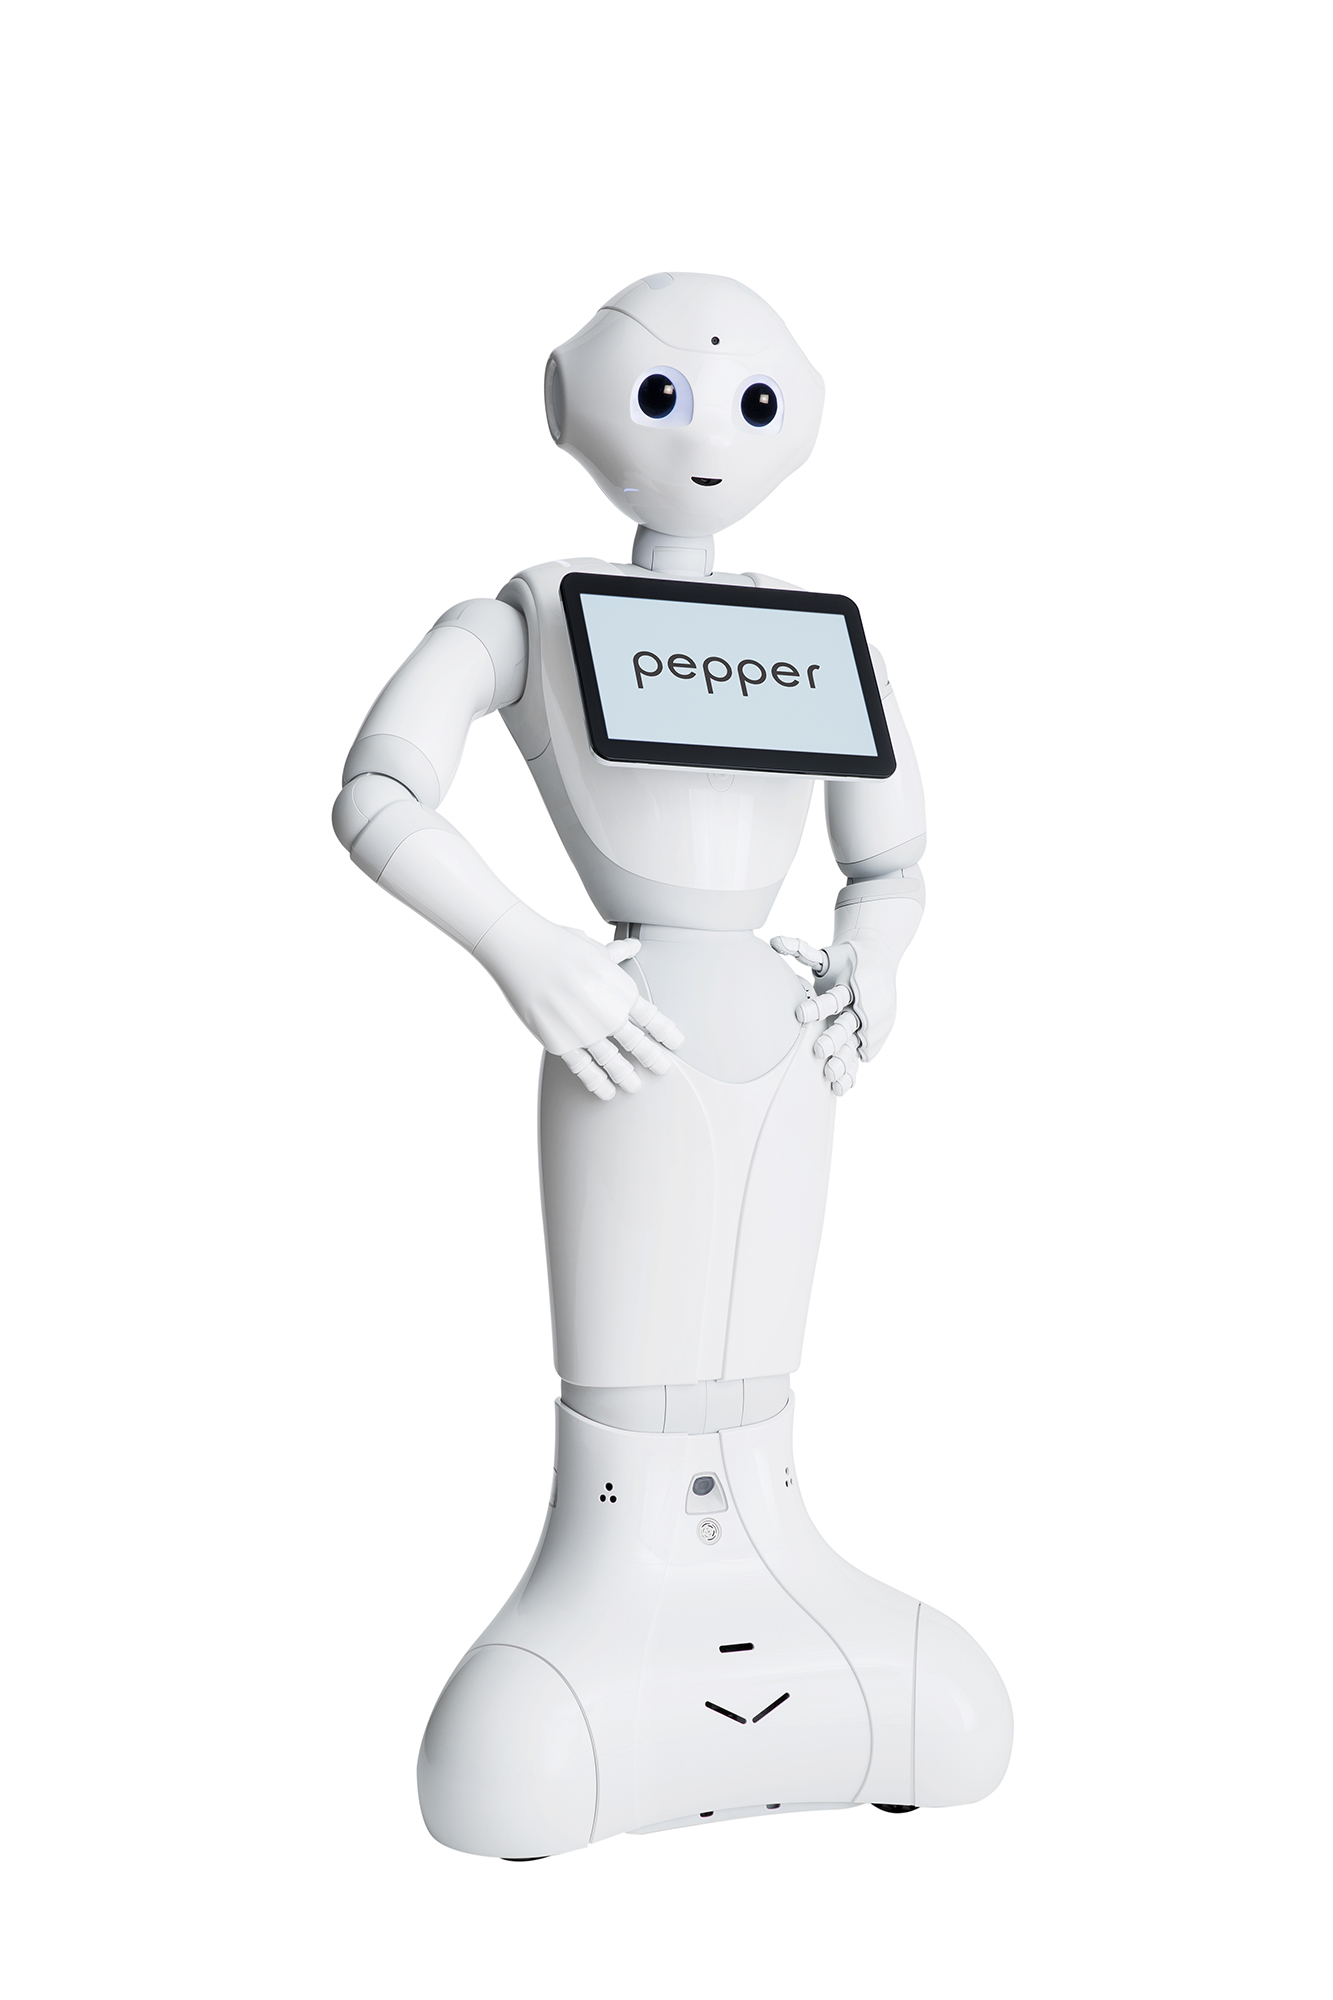
\includegraphics[width=0.8\linewidth]{images/pepper}
			\caption{Pepper, an autonomous humanoid capable of performing on board processing and reaction to external stimuli on a human way.}
			\label{fig:1_pepper}
		\end{subfigure}
		\caption{Robots of each described kind.}
		\label{fig:1_robots}
		
	\end{figure}

The important advances on the last decades on the image processing and audio recognition fields have impulsed the development of assistance systems, apart from critical machines as the previously described examples. \\

This way, several applications have arisen on people recognition and conversational behaviors, and it has been spread to everyday purposes, from personal assistants\footnote{\href{https://www.standard.co.uk/tech/google-smart-home-future-stay-a3868591.html}{Google Smart Home}}, to autonomous driving\footnote{\href{https://electrek.co/2018/06/18/what-tesla-autopilot-see-understand/}{Tesla Autopilot}}.\\


\section{Deep Learning}
\subsection{Machine Learning on Computer Vision}
Almost every time, the desired behavioral is one or more deliberated or reactive responses\footnote{A \emph{deliberated} response implies a certain level of \emph{extra intelligence}. It figures out which could be the best action to perform, considering present, past and probably future information to make the decision.\\ On the other hand, a \emph{reactive} response makes an immediate decision, depending just on what has been just perceived.}, triggered by a certain input (typically perceived by on-board sensors, among others). This raw data, which is typically retrieved on a simple way (images, audio), is processed and mapped into a concrete response. At this point, we can bring up the key question: \emph{how do we process the raw input to obtain a suitable action for the current requirements, or needings?} The answer for that question is \textit{machine learning}: the computer science field that pursues the capacity of machines to learn the suitable response to a previously unknown input. This is achieved by performing a training with a dataset of examples, which need to be properly formatted: the system has to previously know what to look for and evaluate, what is typically called \textit{features}, and learn the proper parameters for an optimum output.\\

Generally, machine learning applications on image processing can be split into two types of response (\autoref{fig:1_class_vs_det}):

\begin{itemize}
	\item \textbf{Classification:} given a set of possible classes $\{c_1, c_2, ..., c_n\}$ to which an image $x_i$ can belong, we select the class $c_i$ where $x_i$ fits the best, given a set of features extracted from it.
	\item \textbf{Detection}: given an image $x_i$, we decide if we can find or not an object/region inside of it which fits into the searched type. In the affirmative case, we locate it (using a region or a bounding box).
\end{itemize}

\begin{figure}[h!]
	\centering
	\begin{subfigure}[h!]{0.7\textwidth}
		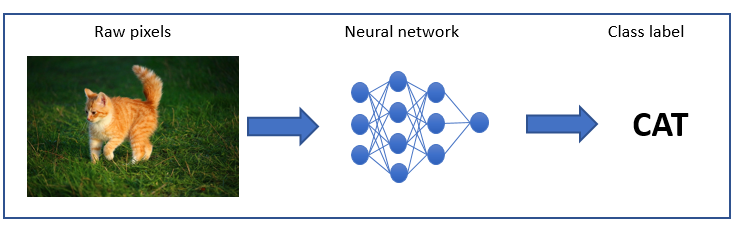
\includegraphics[width=\textwidth]{images/classification}
		\caption{Classification}
		\label{fig:1_classification}
	\end{subfigure}
	
	\qquad
	
	\begin{subfigure}[h!]{0.7\textwidth}
		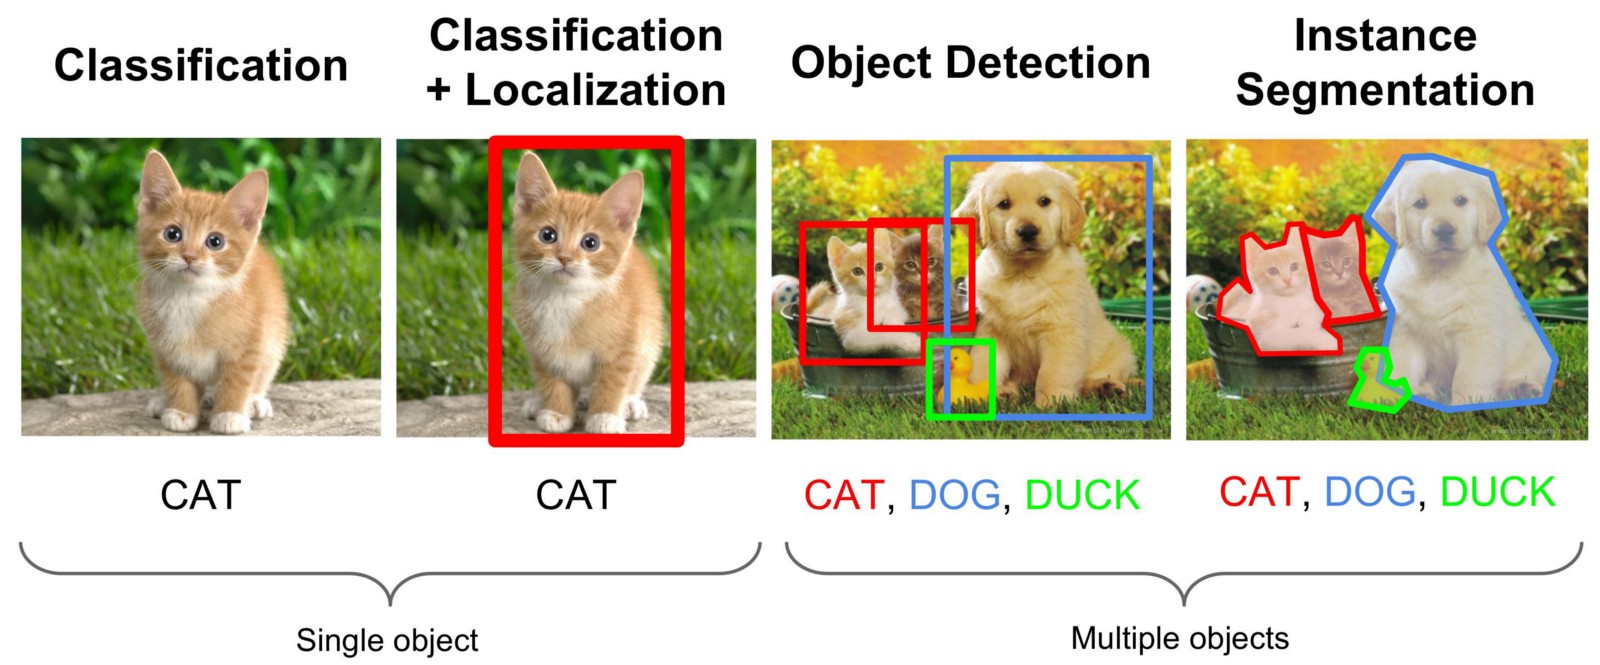
\includegraphics[width=\textwidth]{images/detection}
		\caption{Detection}
		\label{fig:1_detection}			
	\end{subfigure}
	
	\caption{Functional difference between \textit{classification} and \textit{detection}.}
	\label{fig:1_class_vs_det}
\end{figure}


\subsection{Neural Networks}
This has turned deep learning into the cornerstone of current \emph{AI} applications, which don't need complex dataset with a lot of preprocessing (that require important human effort) anymore. That simplicity is achieved through the use of \emph{Neural Networks}. A Neural Network is the representation of an algebraic algorithm which implements non-linear calculus models \cite{dl-nature}. It is composed by several processing \textit{layers}, which are made up of \emph{perceptrons}, that are generally called \textit{neurons}. This is because these neural structures \textit{emulate the human brain}, formed by a huge set of interconnected neurons, which are disposed on the already mentioned layers (\autoref{fig:1_neural_network}).\\

\begin{figure}[htpb]
	\centering
	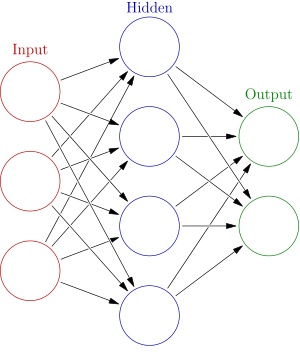
\includegraphics[width=5.5cm]{images/neural_network}
	\caption{Structure of a Neural Network}
	\label{fig:1_neural_network}
\end{figure}

First approaches to neural networks, according to \cite{nn-history} were developed on the 50s-60s decades. This was when the computational potential allowed to develop on a real machine the first modeling of the way it was believed that a brain neuron works, which was inspired by electrical circuits. These experiments \cite{first-neuron} were performed by the neurophysiologist W. McCulloch and the mathematician W. Pitts. Later, in 1949, Donald Hebb \cite{hebb} observed that the synaptic path between two neurons is reinforced (its efficiency rises up) every time it is used. This introduced the concept of \textit{training} on a neural network.

\subsection{Processing unit: the perceptron (neuron)}
\begin{figure}[h]
	\centering
	\begin{tikzpicture}
	\node[functions] (center) {};
	\node[below of=center,font=\scriptsize,text width=4em] {Activation function};
	\draw[thick] (0.5em,0.5em) -- (0,0.5em) -- (0,-0.5em) -- (-0.5em,-0.5em);
	\draw (0em,0.75em) -- (0em,-0.75em);
	\draw (0.75em,0em) -- (-0.75em,0em);
	\node[right of=center] (right) {};
	\path[draw,->] (center) -- (right);
	\node[functions,left=3em of center] (left) {$\sum$};
	\path[draw,->] (left) -- (center);
	\node[weights,left=3em of left] (2) {$w_2$} -- (2) node[input,left of=2] (l2) {$x_2$};
	\path[draw,->] (l2) -- (2);
	\path[draw,->] (2) -- (left);
	\node[below of=2] (dots) {$\vdots$} -- (dots) node[left of=dots] (ldots) {$\vdots$};
	\node[weights,below of=dots] (n) {$w_n$} -- (n) node[input,left of=n] (ln) {$x_n$};
	\path[draw,->] (ln) -- (n);
	\path[draw,->] (n) -- (left);
	\node[weights,above of=2] (1) {$w_1$} -- (1) node[input,left of=1] (l1) {$x_1$};
	\path[draw,->] (l1) -- (1);
	\path[draw,->] (1) -- (left);
	\node[weights,above of=1] (0) {$w_0$} -- (0) node[input,left of=0] (l0) {$1$};
	\path[draw,->] (l0) -- (0);
	\path[draw,->] (0) -- (left);
	\node[below of=ln,font=\scriptsize] {inputs};
	\node[below of=n,font=\scriptsize] {weights};
	\end{tikzpicture}
	\caption{Diagram of a perceptron/neuron}
	\label{fig:1_perceptron}
\end{figure}

\vspace{0.3in}
Every neuron is composed by an structured schema:
\begin{enumerate}
	\item \emph{Inputs}: the data which come into the neuron. It might come from the main stimuli, or from another neuron (as the output of the previous layer). The input for a specific neuron is called its \emph{receptive field} (which region of the total input that stimulates that particular neuron, where it looks for features).
	\item \emph{Weights}: the tuned parameters of the network. They represent the importance given to each feature on that singular neural unit. The weight $w_n$ multiplied $x_n$ times results on the contribution of the feature $n$ in the current neuron. 
	\item \emph{Sum}: the product of all the inputs with their suitable weight come into a sum operation\footnote{We consider $w_0$ as the product to the constant input $1$, as the intercept term (a constant always present independently of the current input).}, to \textit{build a total linear response:} $ z = \sum_{i=0}^{n}x_i \cdot w_i$  \footnote{There is also a summation bias term on each neuron, $b_i$, but it is ignored here for the sake of simplicity, as the weights are more representative with respect to the input.}.
	\item \emph{Activation function}: this is an crucial part of a neural network. Until now, all the numerical computations we have performed were just linear operations. If we keep the output of the neuron being a linear function of the input, we will lose the effect of having more than 1 layer, as really the total result of all the network is a linear function of the first input, so \emph{we could simplify all the network down to one single neuron}. \\
	
	For this reason, we use a \textit{non-linear activation function}, which breaks the linearity on the pipeline to provide the absolute non-linearity followed by the human brain. A typical function is the one called \emph{ReLU} (REctified Linear Unit) \cite{relu}, which follows the formula:
	\begin{equation}
		g(z) = max(0, z)
		\label{eqn:1_relu}
	\end{equation}
	
	\item \emph{Output}: when the activation function has been computed, it is forward-propagated to the output, or to the neurons belonging to the next layer. It can be seen as the importance that particular feature will have on the next neuron: if it takes nearly zero values, the next neuron will be poorly stimulated. There lies the meaning of the name of the previous component: \emph{activation function}.\\
	
	As a conclusion, we can find that the general output of a neuron $a(z)$ as:
	\begin{equation}
		a(z) = g(\sum_{i=0}^{n}x_i \cdot w_i)
	\end{equation}
	
	This will be the new data (\emph{receptive field}) that will be introduced on a neuron or set of them from the next layer.
\end{enumerate}

\subsection{Deep Neural Networks}

\emph{Deep learning} is the piece of machine learning that is capable to \textit{automatically learn the features that the system could use from primary data} (pixels on images, samples on audio, words in text processing, etc.).\\

The fact of having more than one layer gives to the network the concept of \emph{depth}. This opens the door to a vast set of possibilities, as \textit{it allows us to perform deep learning with neural networks: Deep Neural Networks}. This can be achieved, as we can see on \autoref{fig:1_deep_nn}, by introducing a new kind of layer, where all the new neurons are connected to every single neuron of the previous one.\\
This is typically called a \textit{fully connected layer}, and the fact of relating every single activation from the previous layer with a set of tunable weights on each neuron allows to rapidly find common patterns followed by features seen on one of the analyzed scenarios (e.g. syntactical relationships between several kinds of words in language processing, or finding edges or shapes on image detection/classification).

\begin{figure}[h]
	\centering
	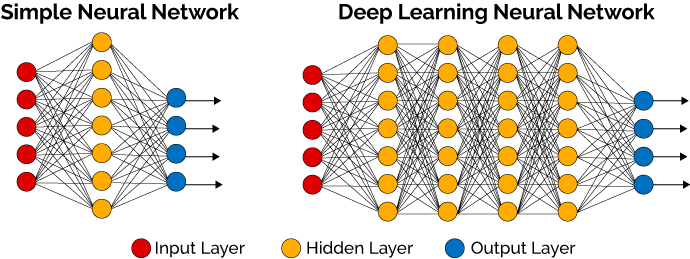
\includegraphics[width=0.9\linewidth]{images/deep_neural_network}
	\caption{Evolution to a \textit{deep} neural network.}
	\label{fig:1_deep_nn}
\end{figure}

\subsection{Convolutional Neural Networks (\emph{CNNs})}
\label{sec:1_cnn}

Finally, this leads us to the last concept we will study on this dissertation. As we have said before, we can connect a big set of neurons between themselves to extract more abstract and complex features, of increasing interest with the number of neurons and layers.\\
 
If we aim to apply this processing to images (\textit{Computer Vision}), we have to take into account that, if we want to input an image into a neural network, each pixel has to be taken as an input, and also the fact that an RGB image is composed of 3 channels (1 channel per color), so, for an image with a dimensions of $m$ pixels wide and $n$ pixels high, we will need $m\cdot n \cdot 3$ input neurons. Besides this considerable number, we will have to take into account the neurons resulting on the additional deeper layers that we will add to have an high enough abstraction level for our application. This drives to absurd numbers of simultaneous neurons working, that are difficultly handable during a feed-forward execution, but absolutely unfeasible on a training process. An additional problem can be a moving object/region on the image: we must be capable to detect the shape of a car on the right side of the image, or in the left one.\\

We can solve both problems simultaneously with an easy procedure: we will not process the entire image at one time. Instead of that \textit{we will perform a convolution operation (\autoref{fig:1_convolution}) between the inputs of our network, and different regions of the image}, sliding and multiplying a \emph{parameterized mask} along the whole image. This operation is performed with the objective of the product returning a high value on the interesting regions of the image. This will output \emph{activation maps}, which symbolize the response of that portion of the image to the weight mask. This can be performed, as we have said before, a few times with different masks to obtain features with a higher degree of abstraction. As we want to keep the computational complexity low, we can alternate these layers with \textit{pooling layers}, which subsample the resulting maps, to keep it simple (if we keep only 1 of each 3 pixels of an activation map, selecting it carefully to retain the maximum information, we can reduce the number of necessary neurons on the next layer on a factor of $\frac{1}{3} \cdot \frac{1}{3} = \frac{1}{9}$). This is reflected on \autoref{fig:1_cnn}, where the process of convolution-pooling can be repeated a few times, and then the result (which should not have considerably big dimensions) are inputted into a fully connected layers, to extract and handle the relations between the features and the possible classes (on a classification scenario).\\


\begin{figure}[h]
	\centering
	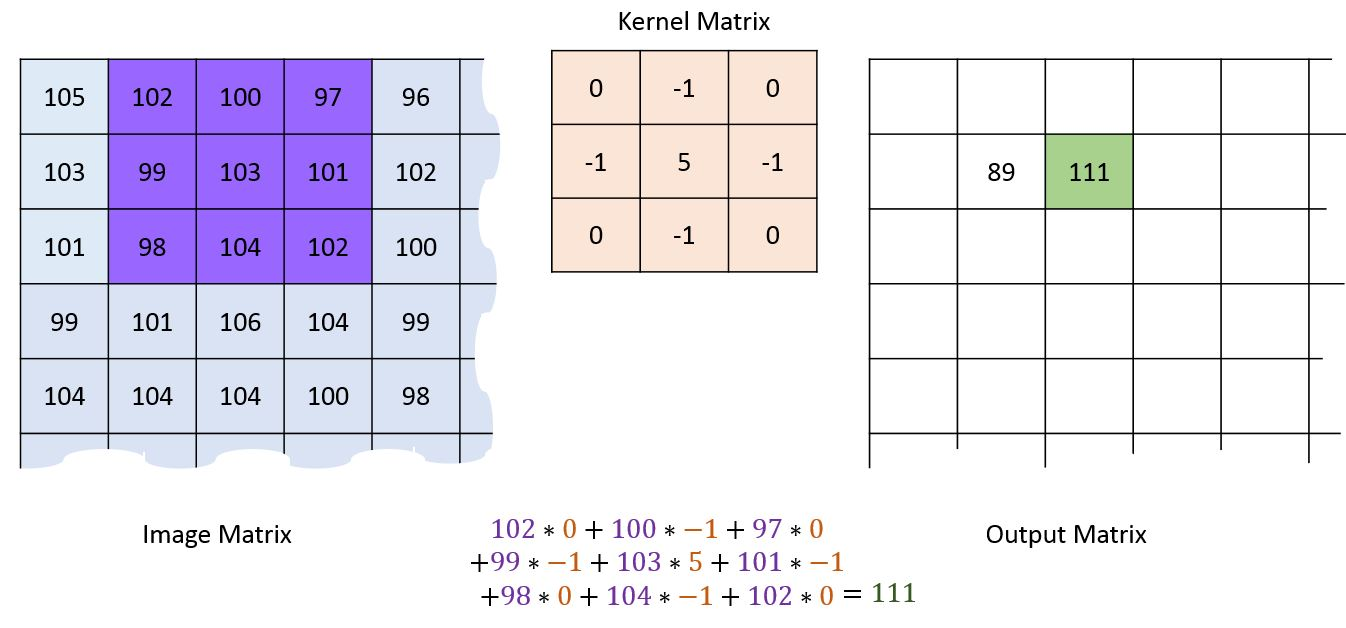
\includegraphics[width=5in]{images/convolution}
	\caption{Convolution operation applied on an image (image from \cite{image-convolution}).}
	\label{fig:1_convolution}
\end{figure}





But, \emph{how do we find the best value for each weight, and for each layer?} That's the process we call \textit{training a network}. Using a technique called \emph{back propagation}, we can compute the most suitable values for every neuron in the network.\\

\begin{figure}[h]
	\centering
	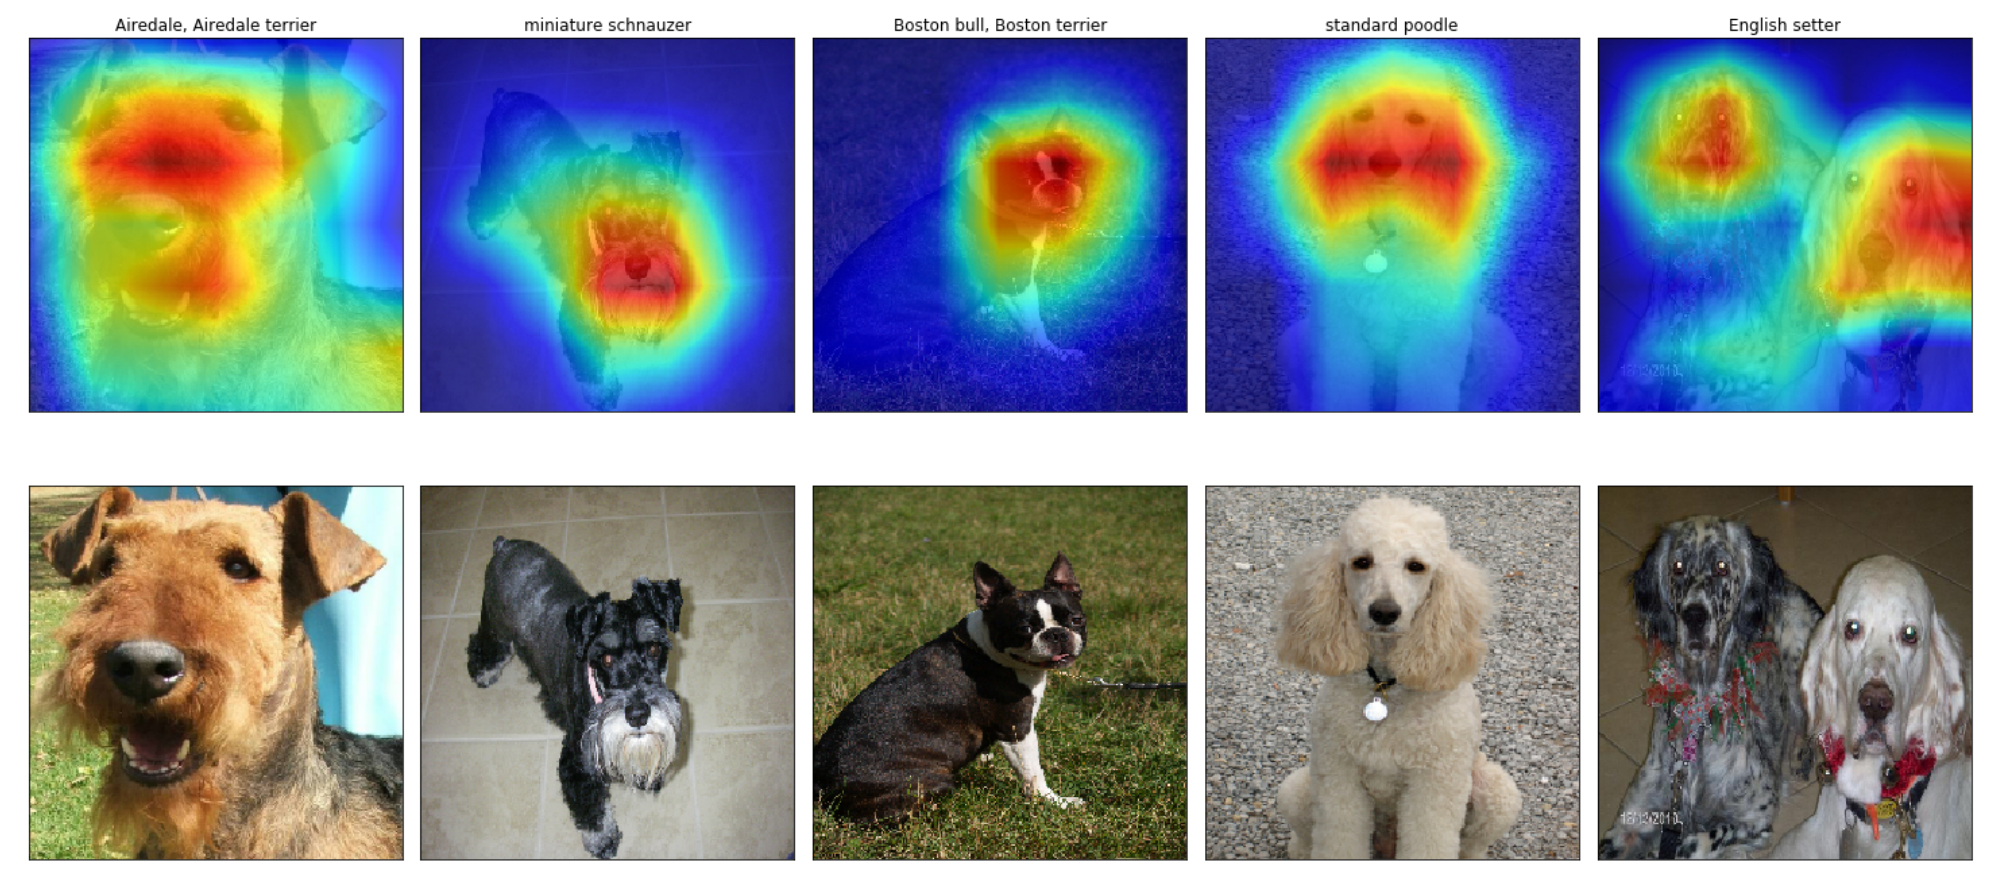
\includegraphics[width=0.9\linewidth]{images/activation_maps}
	\caption{Activation maps of a detection CNN searching for dogs on different images \cite{activation-maps}.}
	\label{fig:1_activation_maps}
\end{figure}



\begin{figure}[h]
	\centering
	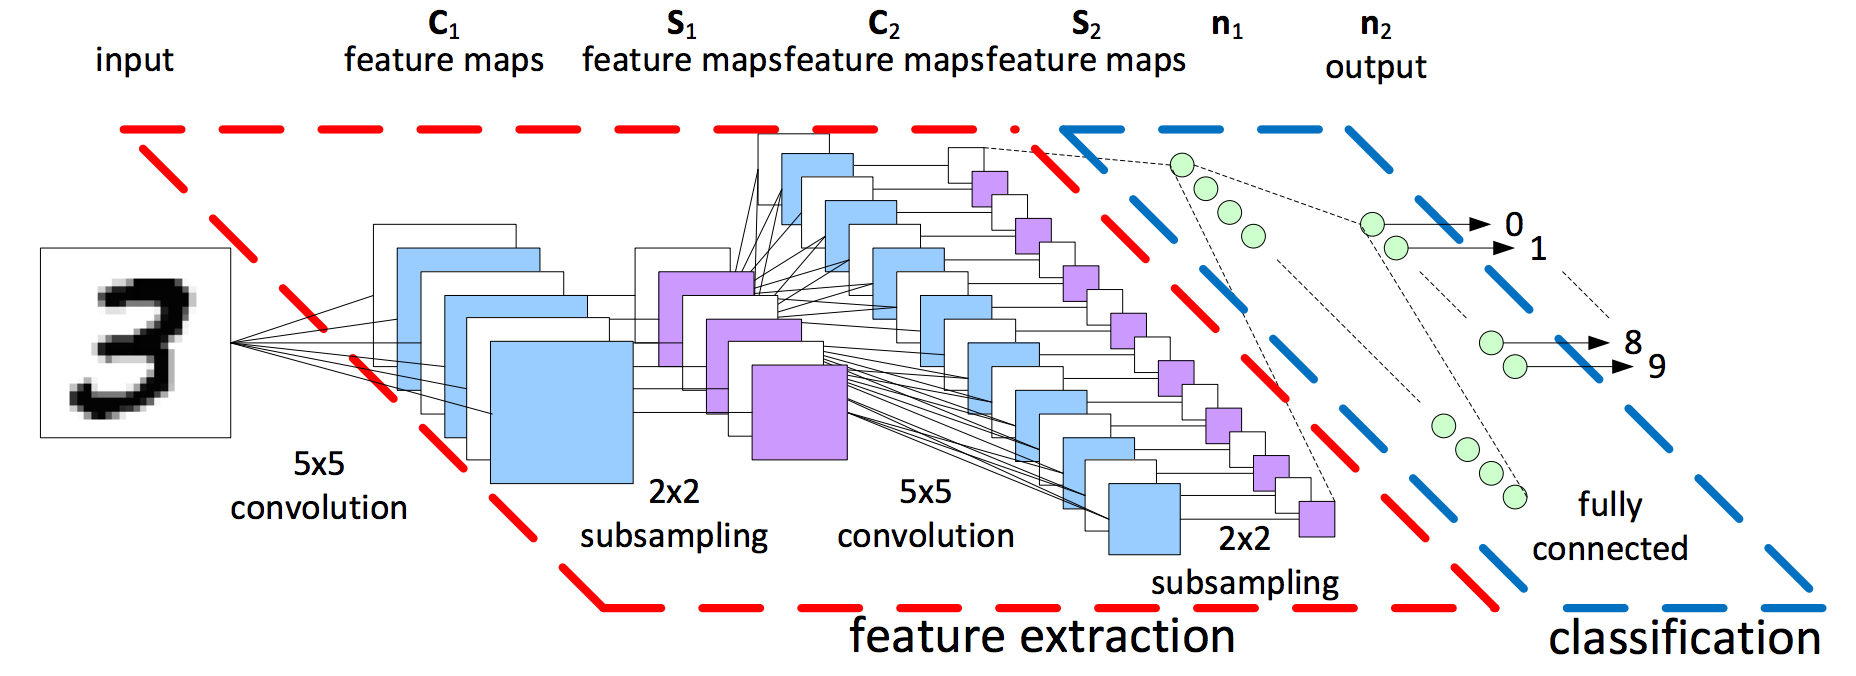
\includegraphics[width=0.9\linewidth]{images/cnn}
	\caption{Schematic of a CNN.}
	\label{fig:1_cnn}
\end{figure}

\section{Deep Learning on JdeRobot}
\label{sec:dl_jderobot}
So, as we have been describing, Deep Learning can be of a great interest on the image processing field, as it allows to implement an easy and really robust AI algorithm.\\

JdeRobot\footnote{\url{https://jderobot.org}} is an open-source software development suite, built from  this University, and among all the developed software/investigation inside it, we can find some interesting programs/projects for our purposes:

\begin{itemize}
	\item \texttt{Detection Suite}\footnote{\url{https://github.com/JdeRobot/dl-DetectionSuite}}: it is a C++ application, suitable to load/benchmark \textit{detection} Darknet/YOLO\footnote{\url{https://pjreddie.com/darknet/}} models, against different databases. It is also capable, through a Python$\rightarrow$C++ interface, to load TensorFlow/Keras models as well.
	
	\begin{figure}[h]
		\centering
		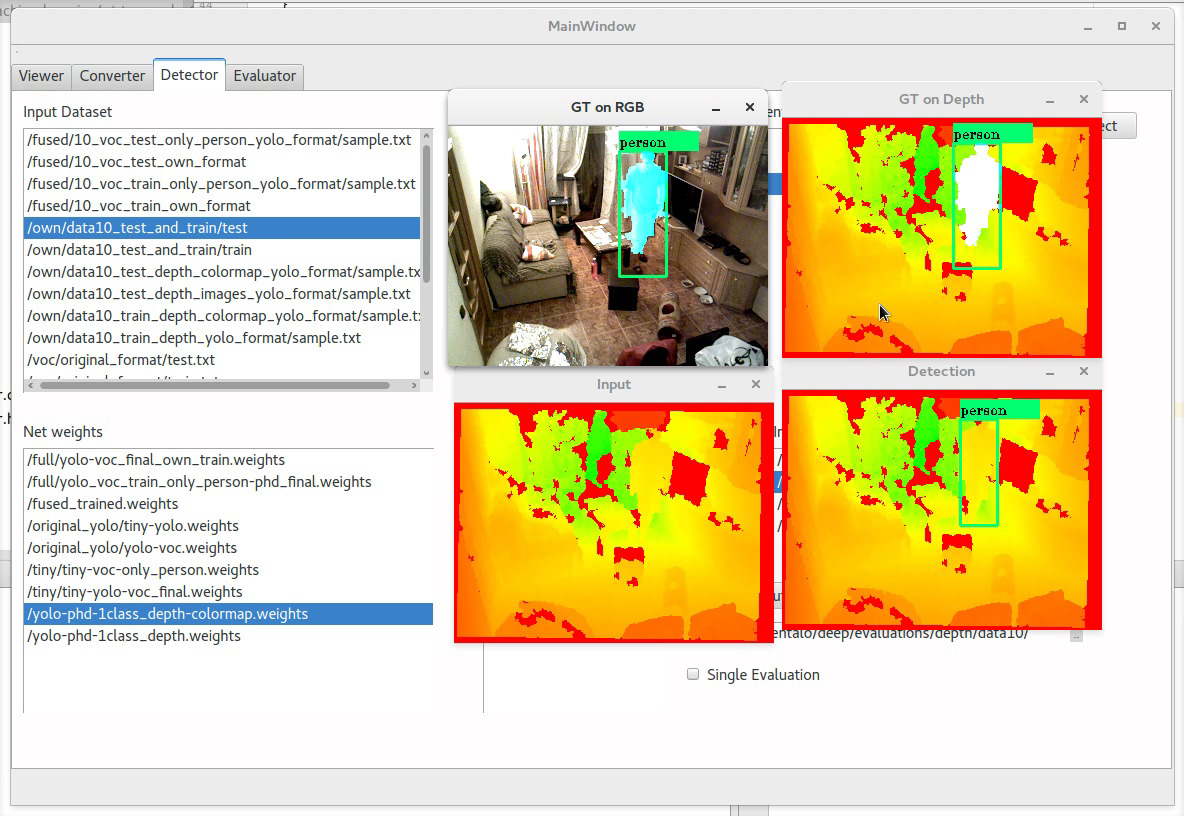
\includegraphics[width=4.5in]{images/detection_suite_depth}
		\caption{\texttt{DetectionSuite} on action.}
		\label{fig:1_detectionsuite}
	\end{figure}

	\item Final project of David Pascual \cite{dpascualhe} and Nuria Oyaga \cite{noyaga}: a further study of Deep Learning, applied on Python (Keras and Caffe frameworks, respectively) to \textit{digit classification} (\autoref{fig:1_digitclassifier}) implementing a CNN as it has been seen.
	
	\begin{figure}[h]
		\centering
		\begin{subfigure}[h]{0.45\linewidth}
			\centering
			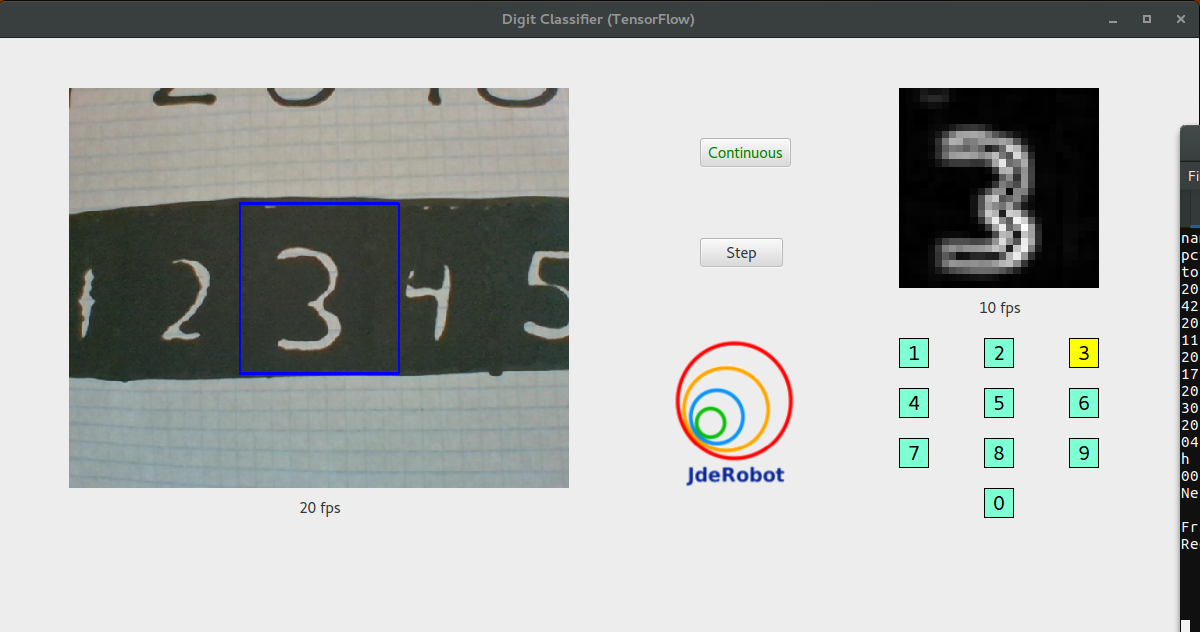
\includegraphics[width=2.7in]{images/digitclassifier}
			\caption{\texttt{DigitClassifier} working.}
			\label{fig:1_digitclassifier}
		\end{subfigure}
		\qquad
		\begin{subfigure}[h]{0.45\linewidth}
			\centering
			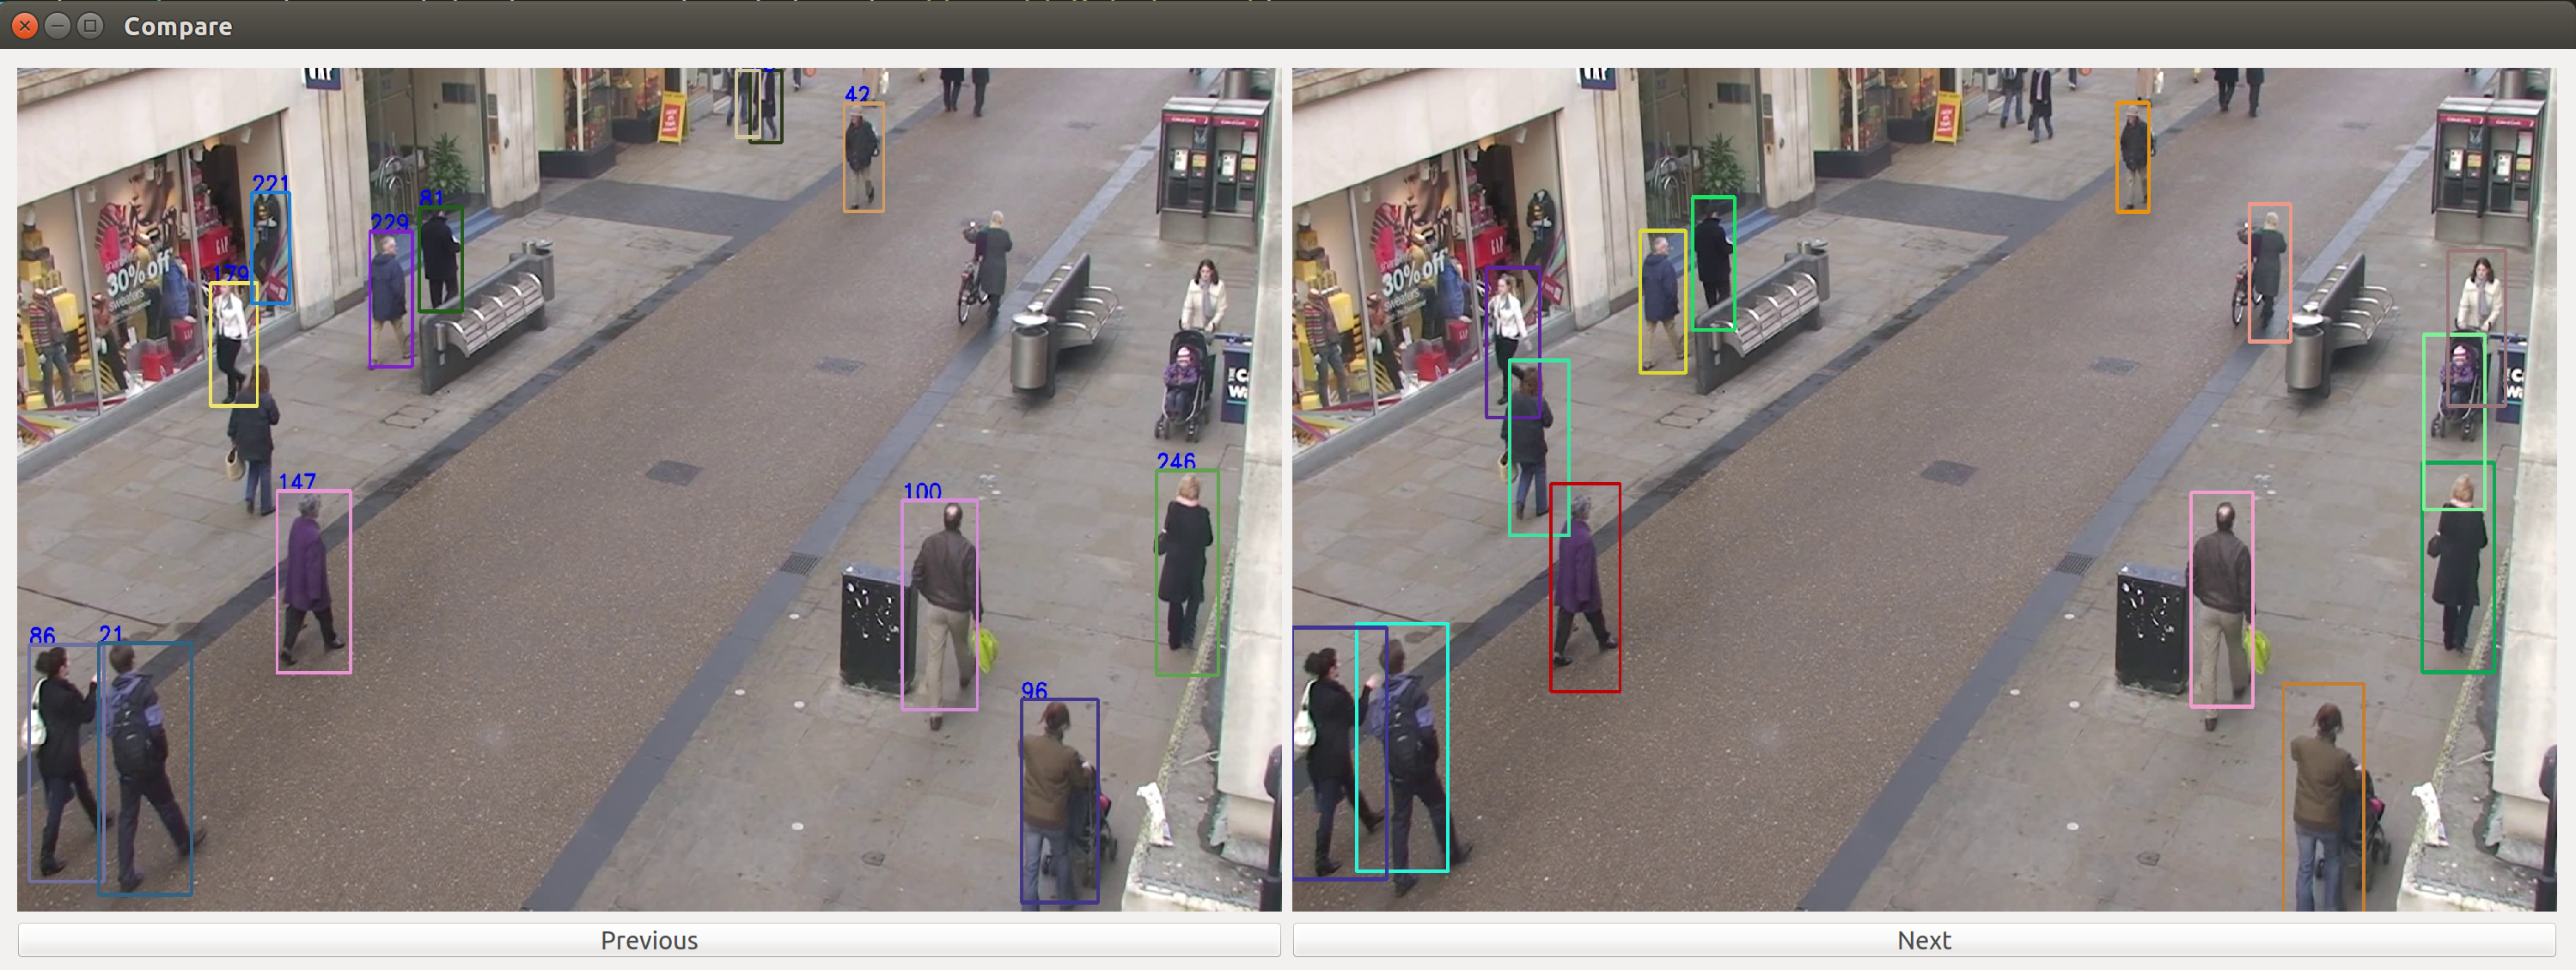
\includegraphics[width=3.7in]{images/marcos_people_tracker}
			\caption{\texttt{PeopleTracker} working.}
			\label{fig:1_people_tracker}
		\end{subfigure}
		\caption{Some JdeRobot student projects on action.}
		\label{fig:1_jderobot_projects}
	\end{figure}

	\item MsC project of Marcos Pieras \cite{marcospieras}: On this master thesis, an application implementing two neural networks (as we will do) has been developed. One of them allows us to \textit{detect} people on an image, and the other one (a siamese network, as we will describe later) can track features of each person, to keep every detected individual identified on a surveillance image system (and possibly trace the route followed by each person) (\autoref{fig:1_people_tracker}).
\end{itemize}

In conclusion, as we have been mentioning and been taking a glance on the possible applications, Deep Learning can make such a brilliant tandem along with a reactive behavioral. We have taken a glance on a few possible applications, and the following dissertation will struggle to demonstrate it.\\




\begin{center}
	\textbf{Robotics + deep learning rock!}
\end{center}


